\section{Code Management}
\label{app:firstApp}

Coding in a programming language is a process of trial-and-error, leading to a working control program or modelling code in many incremental steps. When working on this individually, but more so when coding in a team of code contributors, tracking progress is mandatory. Also, keeping track of the coding progress in multiple locations reduces the risk of information or code losses.

\subsection{Github or Bitbucket account}
\label{appendix::account}

For optimal collaboration, programmers communicate their last achievement to their colleagues or key users by \textit{committing} them in a \textit{repository} on their local PC, then \textit{pushing} the changes to a central copy of the repository in the cloud. Before starting their work, colleagues can \textit{pull} the last changes, so that their local copy of the repository is up-to-date. The updated local copy is then used for adding new contributions or trying out the updated features. Changes or improvements can be committed locally and pushed to the cloud repository by each member of the team.

For establishing a team and implementing the workflow above, each contributor must have an account on a Git repository cloud service.

\begin{itemize}
	\item Github: Go to \url{https://github.com/} and \emph{sign up} with the button in the upper right corner of the web page.
	\begin{figure}[H]
		\centering
		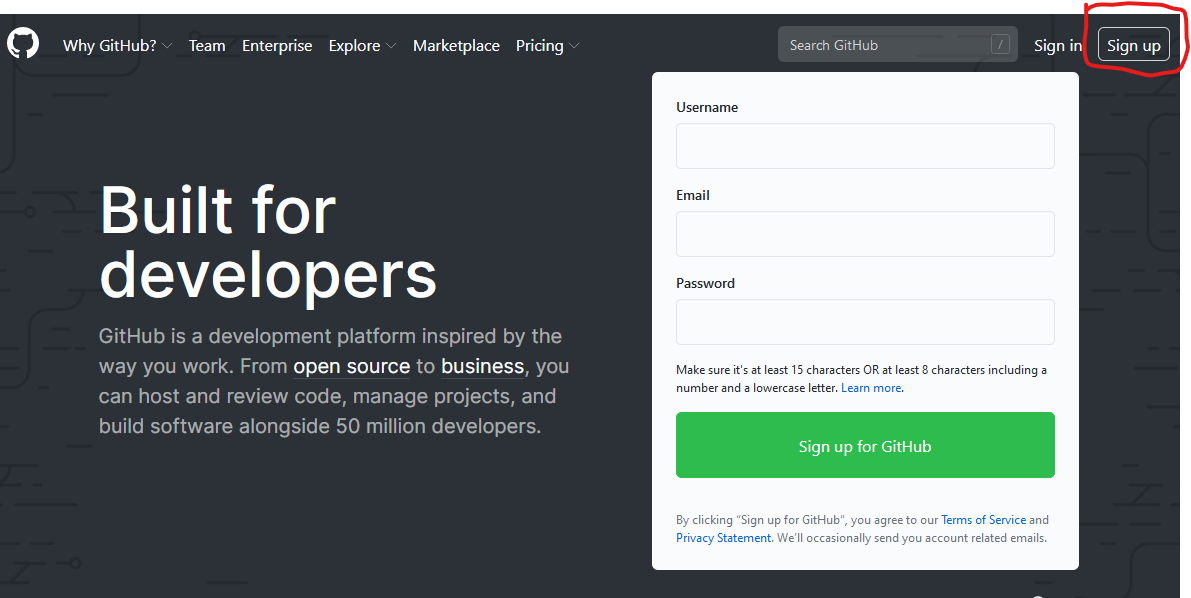
\includegraphics[width=3.0in]{Figures/GitHub_signup.png}
		\caption{GitHub sign-up}
		\label{GitHubSignup}
	\end{figure} 
	\item Bitbucket: Go to \url{https://bitbucket.org/} and sign up with the "Get it free" button in the upper right corner of the web page.
	\begin{figure}[H]
		\centering
		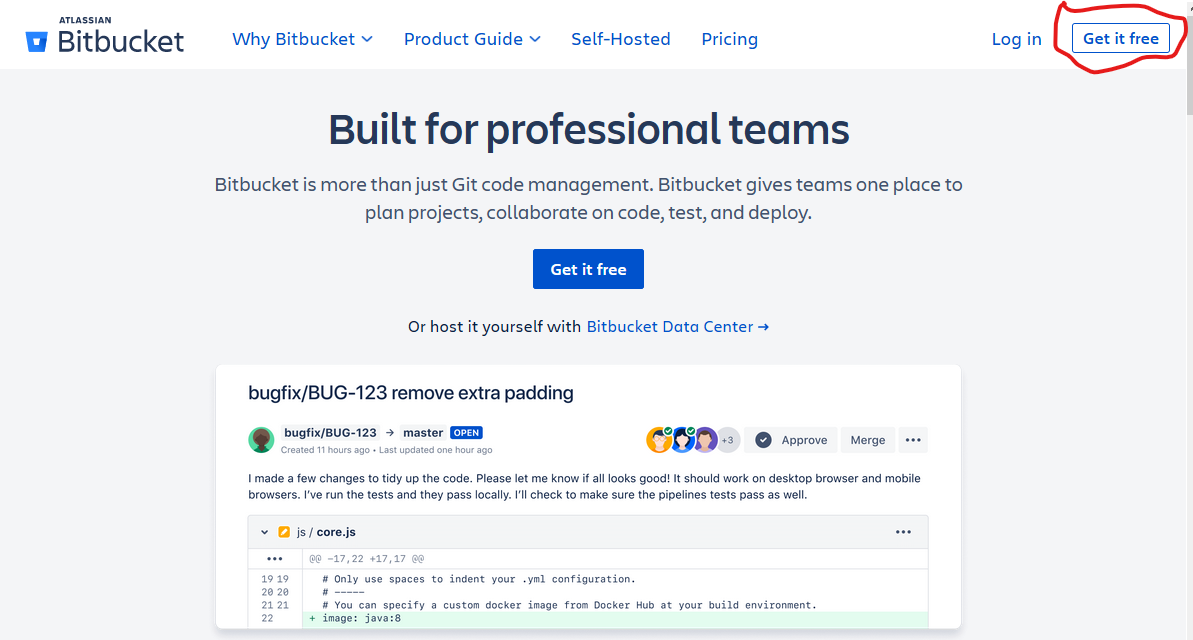
\includegraphics[width=3.0in]{Figures/Bitbucket_signup.png}
		\caption{Bitbucket sign-up}
		\label{BitbucketSignup}
	\end{figure}
\end{itemize}

Do not forget to store your usernames and passwords. The use of a password \textit{vault} is strongly recommended: \url{https://keepass.info/}

\textbf{Note:} Strictly, a GitHub or Bitbucket account is only necessary for all access to \emph{private} repositories or for \emph{contributing} to \emph{public} cloud repositories. Read-only access to \emph{public} repositories is possible without an account.

\subsection{Versioning}
\label{appendix:versioning}

The starting point for version control is the installation of a version control system on your PC. Historically, a number of systems have been invented. Most of them still exist. Among those, CVS, SVN, Bazaar and Mercurial (hg). In the last few years, however, the Git versioning system seems to gain a major "market share". It has been designed by the inventor of Linux, Linus Torvalds, and has a robust performance. The possibilities of Git are a bit overwhelming for the beginning user, which asks for a careful introduction.

\subsubsection{Installation of Git}
On Windows, installation of the \emph{Git for Windows} package is the most convenient option. Download the installer at \url{https://gitforwindows.org/}. 

\begin{figure}[ht]
	\centering
	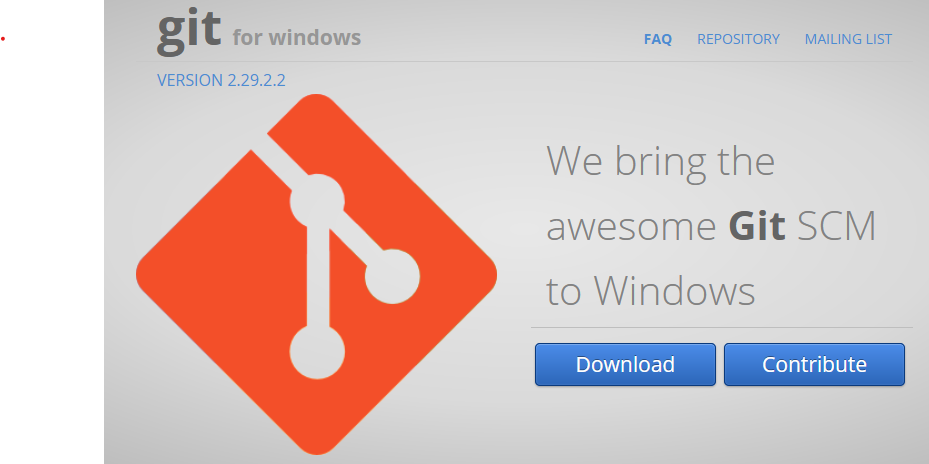
\includegraphics[width=3.0in]{Figures/GitforWindows.png}
	\caption{Git for Windows}
	\label{GitWindows}
\end{figure}

\begin{itemize}
	\item Download the latest version for your OS, which is probably 64-bit \textsf{Git-2.xx.y.z-64-bit.exe}
	\item On execution of the installer, all \emph{default options} can be chosen.
\end{itemize}

On a computer with a Linux OS, there are several options, e.g.:

\begin{itemize}
	\item sudo apt install git (Ubuntu, Debian, RPi)
	\item sudo pacman git (ArchLinux)
\end{itemize}

For Apple Macintosh installation, consult \url{https://git-scm.com/download/mac}.

\subsubsection{Installation of a Git client}

Using Git can be done from the command line (Windows Command Prompt, Git bash or Linux bash). On Linux, this is the preferred option. On Windows, there are useful Git client programs, which make versioning easier after a while. In the beginning, they may just confront you with the overwhelming capacities of Git. Going through this phase merits the effort, however.
A preferred client can be downloaded at \url{https://tortoisegit.org/download/}. 

\begin{itemize}
	\item Download and run the installer: \textsf{TortoiseGit-2.13.0.1-64bit.msi}.
	\item Install with all \emph{default options}.
\end{itemize}

This client integrates with Windows Explorer as an addition to the context menus under the right-mouse-click button.
Installation with the default options is straightforward. Check if the context menus are extended with Git options.

\begin{figure}[ht]
	\centering
	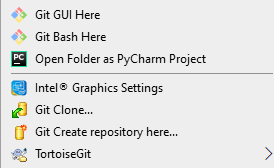
\includegraphics[width=3.0in]{Figures/context_menu.png}
	\caption{Git options in context menu}
	\label{fig:Tortoise_context}
\end{figure}

A second client, with extended functionality can be found at \url{https://www.sourcetreeapp.com/}. Recommended for regular Git users, who work in teams with more than three collaborators, or with collaborators at external reasearch partners. Sourcetree is also available for Mac, but (unfortunately) not for Linux.

\subsubsection{Working with Git}
\label{appendix::gitnotes}

After installation of Git and a Git client, you can start working with Git \emph{repositories}. A repository can be \emph{created} locally, on the harddisk of your PC. Alternatively, a repository from the cloud can be \emph{cloned} to your harddisk. 

After these initial operations, your contributions to the code can be \emph{staged} and \emph{committed} locally and \emph{pushed} to the cloud. Contributions committed and pushed by colleagues can be \emph{pulled} to your local harddisk. 

Regular pulling (before you start coding) and staging-committing-pushing (after you finished coding) cycles will thus assure, that the repositories of all contributors will be synchronized with each other and with the repository in the cloud. The repository in the cloud is often called \emph{origin}.

\textbf{Note:} Each local Git repository should be placed in a separate \emph{local} folder on the physical HDD or SSD. For clarity, it is recommendable to choose a folder name: $\langle repository\_name \rangle$-git. (no spaces in the folder name). 

Each created or cloned repository folder contains a hidden bookkeeping folder named \textsf{.git}. This bookkeeping is not compatible with file sychronization mechanisms. So, please do not create repository folders on Microsoft OneDrive, SharePoint, Teams, Google Drive, OneDrive or SurfDrive shared folders. 

Repository folders are possible on WebDAV, NFS or SMB mounted shared folders, \textbf{if} only one single user has access to the shared folder (from several personal computers, tablets or phones).

\subsection{Git workflow}
\label{appendix:workflow}

\begin{itemize}

\item Creating a repository locally: \url{https://tortoisegit.org/docs/tortoisegit/tgit-dug-create.html}

\item Cloning a repository from GitHub or Bitbucket; \url{https://tortoisegit.org/docs/tortoisegit/tgit-dug-clone.html}

\item Pushing to GitHub or Bitbucket: \url{https://tortoisegit.org/docs/tortoisegit/tgit-dug-push.html}

\item Pulling the changes from the cloud to your local repository: \url{https://tortoisegit.org/docs/tortoisegit/tgit-dug-pull.html}

\item Committing and pushing your local changes to the cloud: \url{https://tortoisegit.org/docs/tortoisegit/tgit-dug-commit.html}
\end{itemize}

\newpage

